\documentclass[tikz,border=6pt]{standalone}
\usepackage{lmodern}
\definecolor{PlotAccent}{gray}{0}
\begin{document}
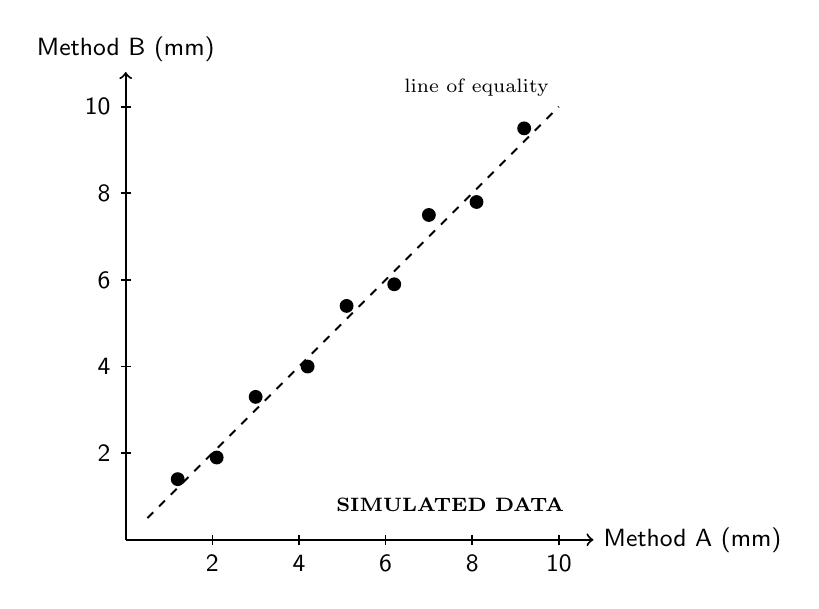
\begin{tikzpicture}[x=0.55cm,y=0.55cm,font=\sffamily\small]
  \draw[->,line width=0.75pt] (0,0) -- (10.8,0) node[right]{Method A (mm)};
  \draw[->,line width=0.75pt] (0,0) -- (0,10.8) node[above]{Method B (mm)};
  \draw[dashed,black,line width=0.65pt] (0.5,0.5) -- (10,10)
    node[above left,font=\scriptsize]{line of equality};
  \foreach \x in {2,4,6,8,10} {
    \draw[line width=0.6pt] (\x,0.12) -- (\x,-0.12) node[below]{\x};
    \draw[line width=0.6pt] (0.12,\x) -- (-0.12,\x) node[left]{\x};
  }
  \foreach \p in {(1.2,1.4),(2.1,1.9),(3.0,3.3),(4.2,4.0),
                   (5.1,5.4),(6.2,5.9),(7.0,7.5),(8.1,7.8),
                   (9.2,9.5)} {
    \fill[PlotAccent] \p circle (2.5pt);
  }
  \node[anchor=south east,font=\bfseries\scriptsize,PlotAccent]
    at (10.35,0.42) {SIMULATED DATA};
\end{tikzpicture}
\end{document}
